\documentclass[12pt]{article}


\usepackage{amssymb, amsmath, amsthm, mathrsfs, multicol, graphicx}

\usepackage{tikz}
\usetikzlibrary{shapes}
\usepackage{pgf}
\usepackage[left=.75in, right=.75in, top=.75in, bottom=0.75in]{geometry}
\usepackage[shortlabels]{enumitem}
 \def\d{\displaystyle}
\def\?{\reflectbox{?}}
\def\b#1{\mathbf{#1}}
\def\f#1{\mathfrak #1}
\def\c#1{\mathcal #1}
\def\s#1{\mathscr #1}
\def\r#1{\mathrm{#1}}
\def\N{\mathbb N}
\def\Z{\mathbb Z}
\def\Q{\mathbb Q}
\def\R{\mathbb R}
\def\C{\mathbb C}
\def\F{\mathbb F}
\def\A{\mathbb A}
\def\X{\mathbb X}
\def\E{\mathbb E}
\def\O{\mathbb O}
\def\U{\mathcal U}
\def\pow{\mathcal P}
\def\inv{^{-1}}
\def\nrml{\triangleleft}
\def\st{:}
\def\~{\widetilde}
\def\rem{\mathcal R}
\def\sigalg{$\sigma$-algebra }
\def\Gal{\mbox{Gal}}
\def\iff{\leftrightarrow}
\def\Iff{\Leftrightarrow}
\def\land{\wedge}
\def\And{\bigwedge}
\def\AAnd{\d\bigwedge\mkern-18mu\bigwedge}
\def\Vee{\bigvee}
\def\VVee{\d\Vee\mkern-18mu\Vee}
\def\imp{\rightarrow}
\def\Imp{\Rightarrow}
\def\Fi{\Leftarrow}

%\def\={\equiv}
\def\var{\mbox{var}}
\def\mod{\mbox{Mod}}
\def\Th{\mbox{Th}}
\def\sat{\mbox{Sat}}
\def\con{\mbox{Con}}
\def\bmodels{=\joinrel\mathrel|}
\def\iffmodels{\bmodels\models}
\def\dbland{\bigwedge \!\!\bigwedge}
\def\dom{\mbox{dom}}
\def\rng{\mbox{range}}
\DeclareMathOperator{\wgt}{wgt}


\def\bar{\overline}


\newcommand{\vtx}[2]{node[fill,circle,inner sep=0pt, minimum size=4pt,label=#1:#2]{}}
\newcommand{\va}[1]{\vtx{above}{#1}}
\newcommand{\vb}[1]{\vtx{below}{#1}}
\newcommand{\vr}[1]{\vtx{right}{#1}}
\newcommand{\vl}[1]{\vtx{left}{#1}}
\renewcommand{\v}{\vtx{above}{}}

\def\circleA{(-.5,0) circle (1)}
\def\circleAlabel{(-1.5,.6) node[above]{$A$}}
\def\circleB{(.5,0) circle (1)}
\def\circleBlabel{(1.5,.6) node[above]{$B$}}
\def\circleC{(0,-1) circle (1)}
\def\circleClabel{(.5,-2) node[right]{$C$}}
\def\twosetbox{(-2,-1.4) rectangle (2,1.4)}
\def\threesetbox{(-2.5,-2.4) rectangle (2.5,1.4)}
\newcommand{\twoline}[2]{\begin{pmatrix}#1 \\ #2 \end{pmatrix}}

\pagestyle{empty}


\begin{document}


\begin{center}
  \textbf{Counting Colorings with PIE}
\end{center}

For any graph $G$, let $P(G,k)$ denote the number of proper colorings of $G$ that use up to $k$ colors (that is, you fix a palete of $k$ colors, and each vertex must be one of those $k$ colors, with different colors for adjacent vertices).  We have previously computed $P(K_5, k)$ and $P(P_5,k)$, and it should be clear how these generalize to any complete graph or path.  What about other graphs?

\begin{enumerate}
  \item For the graph $G$ below, find $P(G,k)$.  You will need to break this up into cases.

  \begin{center}
    {\footnotesize
    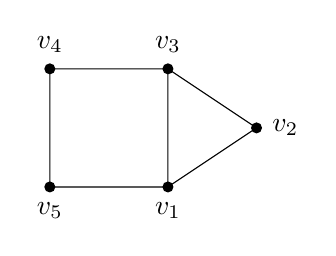
\begin{tikzpicture}[scale=1.5]
      \draw (0,0) \vb{$v_1$} -- (.75, .5) \vr{$v_2$} -- (0,1) \va{$v_3$} -- (-1,1) \va{$v_4$} -- (-1,0) \vb{$v_5$} -- (0,0) -- (0,1);
    \end{tikzpicture}
    }
  \end{center}

\vfill

\item To avoid the case analysis you ran into above, you might try to use the Principle of Inclusion and Exclusion.  You could start by considering \emph{all} colorings of vertices with up to $k$ colors, and then remove those that are not proper.  Before trying this on the graph above, try this for the path $P_3$:

\begin{center}
  {\footnotesize
    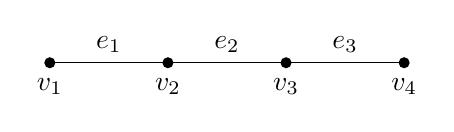
\begin{tikzpicture}[scale=1.5]
      \draw (0,0) \vb{$v_1$} -- (1,0) \vb{$v_2$} -- (2,0) \vb{$v_3$} -- (3,0) \vb{$v_4$};
      \draw (0,0) -- (1,0) node[midway, above]{$e_1$};
      \draw (1,0) -- (2,0) node[midway, above]{$e_2$};
      \draw (2,0) -- (3,0) node[midway, above]{$e_3$};
    \end{tikzpicture}
  }
\end{center}


\vfill
\item Use PIE to find $P(C_5,k)$.  (The graph $C_5$ is the cycle on 5 vertices; label the edges $e_1, \ldots, e_5$ in counter-clockwise order.)

\vfill

\item What happens if you try to use PIE to find $P(G,k)$ for the graph from question 1?

\end{enumerate}



\newpage


\begin{center}
  \textbf{Counting Colorings with Recursion}
\end{center}
Consider two ways to make a graph smaller: you can remove edge $e$ from $G$ (we will call this $G - e$), or you can \emph{contract} the edge $e$, pulling its endpoints together to form one new vertex and removing $e$ (we will call this $G/e$).

\begin{enumerate}
  \item For a fixed value of $k$, which is larger: $P(G,k)$ or $P(G-e,k)$?  How does $P(G/e,k)$ compare with $P(G,k)$?
  \vfill

  \item Prove that for any fixed edge $e$,
  \[P(G-e,k) = P(G,k) + P(G/e,k).\]
  \vfill

  \item We can rearrange this to be a useful recurrence: $P(G,k) = P(G-e,k) - P(G/e,k)$.  Use this to find $P(C_4,k)$ and then $P(C_5,k)$.
  \vfill
  \newpage
  \item Prove that $P(C_n, k) = (k-1)^n + (-1)^n(k-1)$ for $n \ge 3$.  What proof technique would be useful here, given that we have a recurrence relation?
  \vfill
  \item Use the recurrence relation (which is called the \emph{deletion/contraction recurrence}) to find the $P(G, k)$ for our first graph:
  \begin{center}
    {\footnotesize
    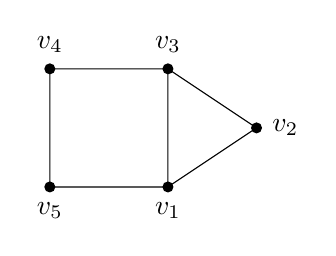
\begin{tikzpicture}[scale=1.5]
      \draw (0,0) \vb{$v_1$} -- (.75, .5) \vr{$v_2$} -- (0,1) \va{$v_3$} -- (-1,1) \va{$v_4$} -- (-1,0) \vb{$v_5$} -- (0,0) -- (0,1);
    \end{tikzpicture}
    }
  \end{center}
  \vfill
\end{enumerate}

\newpage

\begin{center}
  \textbf{The Chromatic Polynomial}
\end{center}

The expressions we have been getting for $P(G,k)$ have been functions of $k$.  But not just any functions: each has been a \emph{polynomial} in the variable $k$.  (We could also consider $P(G,x)$ to make this more explicit).  Thus we call $P(G,k)$ the \emph{chromatic polynomial of $G$}.

\begin{enumerate}
  \item Is $P(G,k)$ really a polynomial for all graphs $G$?  How do you know?
  \vfill

  \item The polynomial $p(x) = x^5 - 5 x^4 + 10 x^3 - 10 x^2 + 4 x$ is the chromatic polynomial for $C_5$.  What can you say about $p(0)$, $p(1)$, and $p(2)$?  What can you say about the function $p(x)$ for $x \ge 3$?
  \vfill
  \item Prove that if $p(x)$ is the chromatic polynomial of a graph with at least one edge, then $(x-1)$ is a factor of $p(x)$.
  \vfill
  \item Let $G$ be a graph with $n$ vertices and $m$ edges.  Prove that $P(G,k)$ is a monic, degree $n$ polynomial, with constant coefficient 0, and that the coefficient of $k^{n-1}$ is $-m$.
  \vfill
  \item Explain how we know that the chromatic polynomial for any \emph{planar} graph is positive on $[4,\infty)$.
\end{enumerate}


\end{document}
